\subsection{\hll{Ornaments from \xmyboxg{$\backslash$pgfornament}}}
%-------------------2.1
\begin{table}[h!]
\begin{tabular}{c | c}
\begin{minipage}[m]{0.4\textwidth}%\enum{\sectionlinetwo{orange}{88}}{2.1}
\begin{tcblisting}{colback=white,colframe=white,comment style={frame hidden,scale=2.1}, comment only, pdf comment, freeze pdf, compilable listing, run pdflatex,}
\documentclass[varwidth, border={10pt 10pt 10pt 10pt}]{standalone}
\usepackage[object=vectorian]{pgfornament}  
\usepackage{tikz}
\begin{document}
\pgfornament[width=5cm]{4} \pgfornament[width=1cm]{5}
\pgfornament[width=1cm]{6} \pgfornament[width=1cm]{7} \pgfornament[width=1cm]{8}
\pgfornament[width=1cm]{9} \pgfornament[width=1cm]{10} \pgfornament[width=1cm]{11}
\pgfornament[width=1cm]{12} \pgfornament[width=1cm]{13} \pgfornament[width=1cm]{14}
\pgfornament[width=1cm]{15} \pgfornament[width=1cm]{16} \pgfornament[width=1cm]{17}
\pgfornament[width=1cm]{18} \pgfornament[width=1cm]{19} \pgfornament[width=1cm]{20}
\pgfornament[width=1cm]{21} \pgfornament[width=1cm]{22} \pgfornament[width=1cm]{23}
\pgfornament[width=1cm]{24} \pgfornament[width=1cm]{25} \pgfornament[width=1cm]{26}
\pgfornament[width=1cm]{27} \pgfornament[width=1cm]{28} \pgfornament[width=1cm]{29} . . .
\end{document}
\end{tcblisting}
\end{minipage}
&
\begin{minipage}[m]{0.55\textwidth}
\renewcommand\textminus{\mbox{-}}%<<<<<<<<<<<
\begin{lstlisting}[numberstyle=\zebra{red!15}{black!10},numbers=left,basicstyle=\ttfamily\footnotesize]{tex}
\documentclass[varwidth]{standalone}
\usepackage[object=vectorian]{pgfornament}  
\usepackage{tikz}

\begin{document}
\pgfornament[width=5cm]{4} \pgfornament[width=1cm]{5}
\pgfornament[width=1cm]{6} \pgfornament[width=1cm]{7} 
\pgfornament[width=1cm]{8} \pgfornament[width=1cm]{9} 
\pgfornament[width=1cm]{10} \pgfornament[width=1cm]{11}
\pgfornament[width=1cm]{12} \pgfornament[width=1cm]{13}
\pgfornament[width=1cm]{14} \pgfornament[width=1cm]{15} 
\pgfornament[width=1cm]{16} \pgfornament[width=1cm]{17}
\pgfornament[width=1cm]{18} \pgfornament[width=1cm]{19} 
\end{document}
\end{lstlisting}
\end{minipage}
\end{tabular}
\end{table}


%-------------------2.2
\subsection{\hll{Wireframe rendering}}
\begin{table}[h!]
\begin{tabular}{c | c}
\begin{minipage}[m]{0.4\textwidth}
\enum{\centering \roboto\huge\contourlength{.15em}
\contour{gray}{boxed} \contour{red}{boxed} \contour{yellow}{boxed}}{2.2}
\end{minipage}
&
\begin{minipage}[m]{0.55\textwidth}
\begin{lstlisting}[numberstyle=\zebra{red!15}{black!10},numbers=left,basicstyle=\ttfamily\footnotesize] 
\documentclass{article}
\usepackage{xcolor}
\usepackage{roboto}
\usepackage[outline]{contour}

\begin{document}
\roboto\huge\contourlength{.15em}
\contour{gray}{boxed}
\end{document}
\end{lstlisting}
\end{minipage}
\end{tabular}
\end{table}
\clearpage

%-------------------2.3
\subsection{\hll{Justifyed text}}
\begin{table}[h!]
\begin{tabular}{c | c}
\begin{minipage}[m]{0.4\textwidth}
\enum{\texttt{\tiny\justify\blindenumerate[10]}}{2.3}
\end{minipage}
&
\begin{minipage}[m]{0.55\textwidth}
\renewcommand\textminus{\mbox{-}}%<<<<<<<<<<<
\begin{lstlisting}[numberstyle=\zebra{red!15}{black!10},numbers=left,basicstyle=\ttfamily\footnotesize] 
\documentclass{article}
\usepackage{blindtext}
\newcommand*\justify{%
  \fontdimen2\font=0.4em% interword space
  \fontdimen3\font=0.2em% interword stretch
  \fontdimen4\font=0.1em% interword shrink
  \fontdimen7\font=0.1em% extra space
  \hyphenchar\font=`\-% allowing hyphenation
}
\begin{document}
\texttt{\justify\blindenumerate[10]}
\end{document}
\end{lstlisting}
\end{minipage}
\end{tabular}
\end{table}


%-------------------2.4
\subsection{\hll{Text under an underline}}
\begin{table}[h!]
\begin{tabular}{c | c}
\begin{minipage}[m]{0.4\textwidth}
\begin{tikzpicture}
\node (0,0) {\begin{minipage}[m]{0.90\textwidth}
  \begin{tcblisting}{colback=white,colframe=white,comment style=
  {frame hidden,scale=2.1}, comment only, pdf comment, freeze pdf, compilable listing, run pdflatex,}
    \documentclass{standalone}
    \usepackage{array}
    \newcommand{\mycommand}[2]{\begin{tabular}[t]{@{} c @{}}
    #1\\  \hline
    #2
    \end{tabular}}
    \begin{document}
    text \mycommand{Some long Text}{text under line} text
    \end{document}
  \end{tcblisting}
\end{minipage}};
\node [opacity=0.05] (0,0) {\scalebox{8.0}{\textcolor{red}{2.4}}};
\end{tikzpicture}
\end{minipage}
&
\begin{minipage}[m]{0.55\textwidth}
\renewcommand\textminus{\mbox{-}}%<<<<<<<<<<<
\begin{lstlisting}[numberstyle=\zebra{red!15}{black!10},numbers=left,basicstyle=\ttfamily\footnotesize] 
\documentclass{standalone}
\usepackage{array}
%\setlength\extrarowheight{2pt}
\newcommand{\mycommand}[2]{\begin{tabular}[t]{@{} c @{}}
#1\\  \hline
#2
\end{tabular}}

\begin{document}
text \mycommand{Some long Text}{text under line} text 
\end{document}
\end{lstlisting}
\end{minipage}
\end{tabular}
\end{table}

%-------------------2.5
\subsection{\hll{Various types of underlining}}
\begin{table}[h!]
\begin{tabular}{c | c}
\begin{minipage}[m]{0.4\textwidth}
%\enum{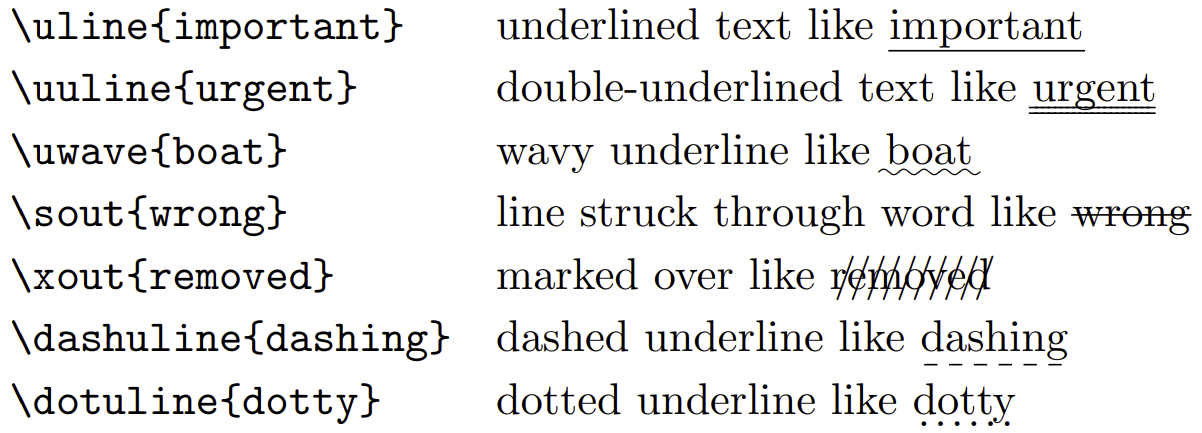
\includegraphics[width=\linewidth]{2.6.png}}{2.5}
\begin{tcblisting}{colback=white,colframe=white,  comment only,  pdf comment,  freeze pdf,  compilable listing,  run pdflatex,
comment style={frame hidden,scale=2}}
\documentclass{standalone}
\usepackage[skins,listings]{tcolorbox}
\usepackage{ulem}
\newtcblisting{exampleB}[2][]{%
width=10cm,  colframe=red!50!yellow!50!black,
colback=white,  coltitle=red!50!yellow!3!white,
bicolor,colbacklower=red!50!yellow!5!white,
fonttitle=\sffamily\bfseries,  sidebyside,text and listing,  title=#2,#1}

\begin{document}
\begin{exampleB}[lefthand width=3.5cm, text outside listing,colback=red!50!yellow!5!white,top=0mm,bottom=0mm,left=0mm,right=0mm,
arc=0mm,boxrule=1pt]{}
Some \uline{important} text\\
Some \uuline{urgent} text\\
Some \uwave{boat} text\\
Some \sout{wrong} text\\
Some \xout{removed} text\\
Some \dashuline{dashing} text\\
Some \dotuline{dotty} text
\end{exampleB}
\end{document}
\end{tcblisting}
\end{minipage}
&
\begin{minipage}[m]{0.55\textwidth}
\renewcommand\textminus{\mbox{-}}%<<<<<<<<<<<
\begin{lstlisting}[numberstyle=\zebra{red!15}{black!10},numbers=left,basicstyle=\ttfamily\footnotesize] 
\documentclass[14pt]{extreport}
\usepackage{ulem}

\begin{document}
\uline{important} \uuline{urgent}
\uwave{boat}      \sout{wrong}
\xout{removed}    \dashuline{dashing} 
\dotuline{dotty} 
\end{document}
\end{lstlisting}
\end{minipage}
\end{tabular}
\end{table}
\clearpage

%-------------------2.6
\subsection{\hll{Bullets Style}}
\begin{table}[h!]
\begin{tabular}{c | c}
\begin{minipage}[m]{0.4\textwidth}
\enum{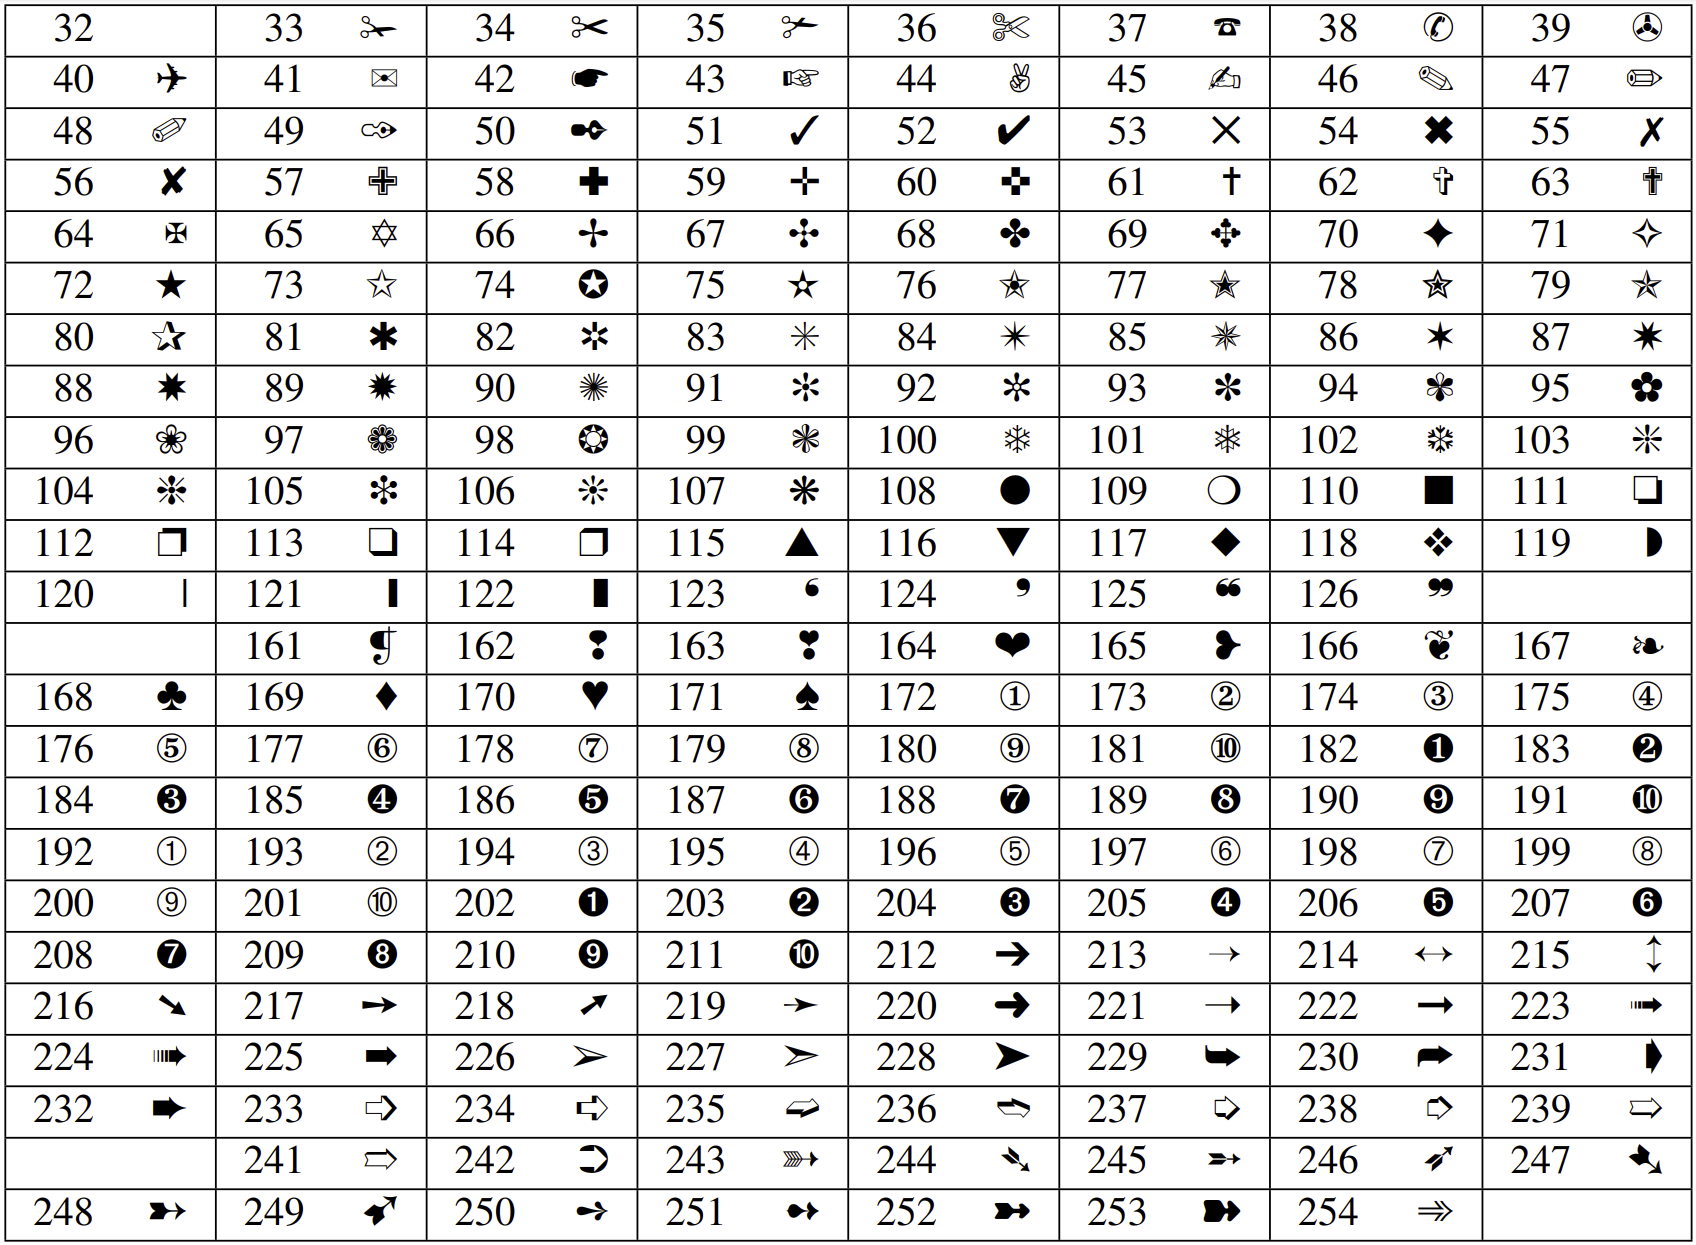
\includegraphics[width=\linewidth]{2.5.png} }{2.6}
\end{minipage}
&
\begin{minipage}[m]{0.55\textwidth}
\renewcommand\textminus{\mbox{-}}%<<<<<<<<<<<
\begin{lstlisting}[numberstyle=\zebra{red!15}{black!10},numbers=left,basicstyle=\ttfamily\footnotesize] 
\documentclass{article}
\usepackage{pifont}

\begin{document}
\begin{itemize}
    \item[\ding{51}] Code 51
    \item[\ding{56}] Code 56
    \item[\ding{43}] Code 43
    \item[\ding{118}] Code 118
    \item[\ding{170}] Code 170
\end{itemize}
\ding{46} \ding{70} \ding{57}  \ding{98} \ding{96}
\end{document}
\end{lstlisting}
\end{minipage}
\end{tabular}
\end{table}

%-------------------2.7
\subsection{\hll{Change the title of \xmyboxg{$\backslash$tableofcontents}}}
\begin{table}[h!]
\begin{tabular}{c | c}
\begin{minipage}[m]{0.4\textwidth}
\enum{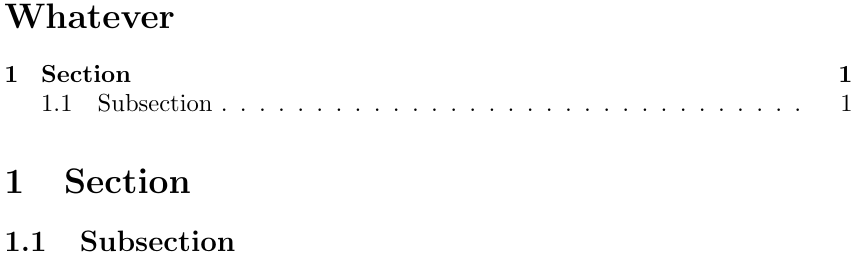
\includegraphics[width=\linewidth]{2.7.png}}{2.7}
\end{minipage}
&
\begin{minipage}[m]{0.55\textwidth}
\renewcommand\textminus{\mbox{-}}%<<<<<<<<<<<
\begin{lstlisting}[numberstyle=\zebra{red!15}{black!10},numbers=left,basicstyle=\ttfamily\footnotesize] 
\documentclass{article}
\renewcommand{\contentsname}{Whatever}

\begin{document}
  \tableofcontents
  \subsection{\hll{Section}
  \subsection{\hll{Subsection}
\end{document}
\end{lstlisting}
\end{minipage}
\end{tabular}
\end{table}


%-------------------2.8
%-------------------2.9
%-------------------2.10
%-------------------2.11
%-------------------2.12


 


